\batchmode
\documentclass[twoside]{article}

% Packages required by doxygen
\usepackage{fixltx2e}
\usepackage{calc}
\usepackage{doxygen}
\usepackage[export]{adjustbox} % also loads graphicx
\usepackage{graphicx}
\usepackage[utf8]{inputenc}
\usepackage{makeidx}
\usepackage{multicol}
\usepackage{multirow}
\PassOptionsToPackage{warn}{textcomp}
\usepackage{textcomp}
\usepackage[nointegrals]{wasysym}
\usepackage[table]{xcolor}

% Font selection
\usepackage[T1]{fontenc}
\usepackage[scaled=.90]{helvet}
\usepackage{courier}
\usepackage{amssymb}
\usepackage{sectsty}
\renewcommand{\familydefault}{\sfdefault}
\allsectionsfont{%
  \fontseries{bc}\selectfont%
  \color{darkgray}%
}
\renewcommand{\DoxyLabelFont}{%
  \fontseries{bc}\selectfont%
  \color{darkgray}%
}
\newcommand{\+}{\discretionary{\mbox{\scriptsize$\hookleftarrow$}}{}{}}

% Page & text layout
\usepackage{geometry}
\geometry{%
  letterpaper,%
  top=2.5cm,%
  bottom=2.5cm,%
  left=2.5cm,%
  right=2.5cm%
}
\tolerance=750
\hfuzz=15pt
\hbadness=750
\setlength{\emergencystretch}{15pt}
\setlength{\parindent}{0cm}
\setlength{\parskip}{0.2cm}
\makeatletter
\renewcommand{\paragraph}{%
  \@startsection{paragraph}{4}{0ex}{-1.0ex}{1.0ex}{%
    \normalfont\normalsize\bfseries\SS@parafont%
  }%
}
\renewcommand{\subparagraph}{%
  \@startsection{subparagraph}{5}{0ex}{-1.0ex}{1.0ex}{%
    \normalfont\normalsize\bfseries\SS@subparafont%
  }%
}
\makeatother

% Headers & footers
\usepackage{fancyhdr}
\pagestyle{fancyplain}
\fancyhead[LE]{\fancyplain{}{\bfseries\thepage}}
\fancyhead[CE]{\fancyplain{}{}}
\fancyhead[RE]{\fancyplain{}{\bfseries\leftmark}}
\fancyhead[LO]{\fancyplain{}{\bfseries\rightmark}}
\fancyhead[CO]{\fancyplain{}{}}
\fancyhead[RO]{\fancyplain{}{\bfseries\thepage}}
\fancyfoot[LE]{\fancyplain{}{}}
\fancyfoot[CE]{\fancyplain{}{}}
\fancyfoot[RE]{\fancyplain{}{\bfseries\scriptsize Generated on Tue Apr 14 2015 15\+:14\+:08 for N\+D\+K by Doxygen }}
\fancyfoot[LO]{\fancyplain{}{\bfseries\scriptsize Generated on Tue Apr 14 2015 15\+:14\+:08 for N\+D\+K by Doxygen }}
\fancyfoot[CO]{\fancyplain{}{}}
\fancyfoot[RO]{\fancyplain{}{}}
\renewcommand{\footrulewidth}{0.4pt}
\renewcommand{\sectionmark}[1]{%
  \markright{\thesection\ #1}%
}

% Indices & bibliography
\usepackage{natbib}
\usepackage[titles]{tocloft}
\setcounter{tocdepth}{3}
\setcounter{secnumdepth}{5}
\makeindex

% Hyperlinks (required, but should be loaded last)
\usepackage{ifpdf}
\ifpdf
  \usepackage[pdftex,pagebackref=true]{hyperref}
\else
  \usepackage[ps2pdf,pagebackref=true]{hyperref}
\fi
\hypersetup{%
  colorlinks=true,%
  linkcolor=blue,%
  citecolor=blue,%
  unicode%
}

% Custom commands
\newcommand{\clearemptydoublepage}{%
  \newpage{\pagestyle{empty}\cleardoublepage}%
}


%===== C O N T E N T S =====

\begin{document}

% Titlepage & ToC
\pagenumbering{roman}
\begin{titlepage}
\vspace*{7cm}
\begin{center}%
{\Large N\+D\+K \\[1ex]\large 2.\+24.\+02.\+31 }\\
\vspace*{1cm}
{\large Generated by Doxygen 1.8.9.1}\\
\vspace*{0.5cm}
{\small Tue Apr 14 2015 15:14:08}\\
\end{center}
\end{titlepage}
\tableofcontents
\pagenumbering{arabic}

%--- Begin generated contents ---
\section{N\+D\+K A\+P\+I Reference}
\label{index}\hypertarget{index}{}\hypertarget{index_modules}{}\subsection{Modules}\label{index_modules}
The following modules are included in this preliminary document\+:
\begin{DoxyItemize}
\item \hyperlink{mytime_8h}{M\+Y\+T\+I\+M\+E}
\item \hyperlink{sntp_8h}{S\+N\+T\+P client (beta)} 
\end{DoxyItemize}
\section{Disclaimer}
\label{_disclaimer}
 
\section{File Index}
\subsection{File List}
Here is a list of all files with brief descriptions\+:\begin{DoxyCompactList}
\item\contentsline{section}{\hyperlink{mytime_8h}{mytime.\+h} }{\pageref{mytime_8h}}{}
\item\contentsline{section}{\hyperlink{sntp_8h}{sntp.\+h} }{\pageref{sntp_8h}}{}
\end{DoxyCompactList}

\section{File Documentation}
\subsection{disclaimer.\+dox File Reference}
\label{disclaimer_8dox}\index{disclaimer.\+dox@{disclaimer.\+dox}}

\subsection{doxygen.\+txt File Reference}
\label{doxygen_8txt}\index{doxygen.\+txt@{doxygen.\+txt}}

\subsection{mytime.\+h File Reference}
\label{mytime_8h}\index{mytime.\+h@{mytime.\+h}}


\subsubsection{Detailed Description}
The M\+Y\+T\+I\+M\+E module uses the S\+Y\+S/\+B\+I\+O\+S Clock module to keep track of system time for hardware platforms that do not have a Real Time Clock.

The module internally tracks the time by keeping count of the number of seconds since the Epoch, which is defined to be January 1, 1970.

Users of the M\+Y\+T\+I\+M\+E module can access its internal time value using supplied getter and setter functions.

\subsubsection*{Example Usage}

The M\+Y\+T\+I\+M\+E module is part of the N\+D\+K nettools library. An application should include its header file as follows\+: 
\begin{DoxyCode}
\textcolor{preprocessor}{#include <ti/ndk/nettools/mytime/mytime.h>}
\end{DoxyCode}


\paragraph*{Initializing The M\+Y\+T\+I\+M\+E Module}

To initialize and start the M\+Y\+T\+I\+M\+E module clock, call the following function\+: 
\begin{DoxyCode}
MYTIME_init();
\end{DoxyCode}


\paragraph*{Getting The Current Time}

The internal time value can be obtained by calling the \hyperlink{mytime_8h_a05f7406d31d93f6dc9b7ecaac8a37376}{M\+Y\+T\+I\+M\+E\+\_\+gettime()} function\+: 
\begin{DoxyCode}
uint32\_t currentTime = MYTIME_gettime();
\end{DoxyCode}


\paragraph*{Setting The Current Time}

The internal time value can be set by calling the \hyperlink{mytime_8h_a0f77aa4bc459ff00050636b47cda79d3}{M\+Y\+T\+I\+M\+E\+\_\+settime()} function\+: 
\begin{DoxyCode}
uint32\_t newTime = 100;
MYTIME_settime(newTime);
\end{DoxyCode}


\paragraph*{Deinitializing The M\+Y\+T\+I\+M\+E Module}

The following function can be called to stop the M\+Y\+T\+I\+M\+E Clock and free its resources\+: 
\begin{DoxyCode}
MYTIME_exit();
\end{DoxyCode}
 

{\ttfamily \#include $<$xdc/std.\+h$>$}\\*
{\ttfamily \#include $<$stdint.\+h$>$}\\*
Include dependency graph for mytime.\+h\+:
\nopagebreak
\begin{figure}[H]
\begin{center}
\leavevmode
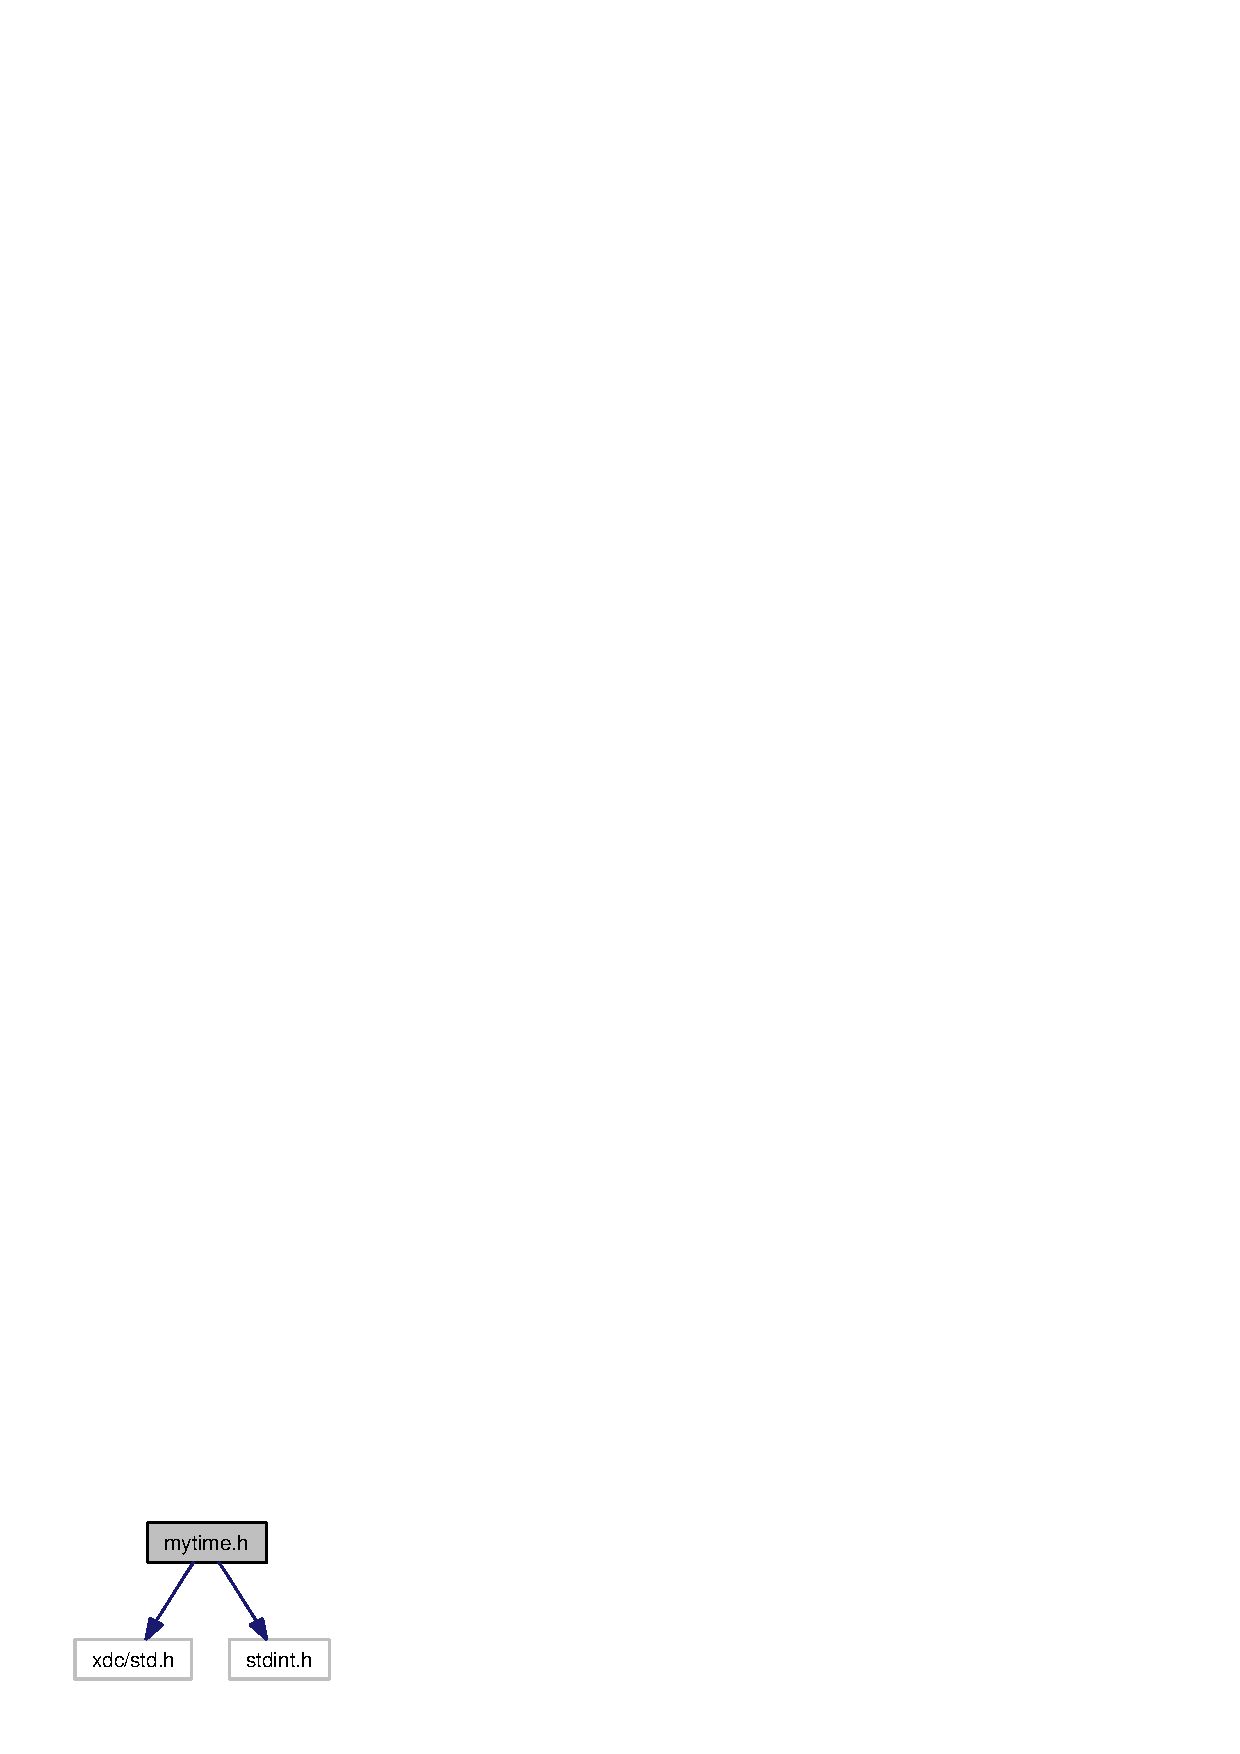
\includegraphics[width=159pt]{mytime_8h__incl}
\end{center}
\end{figure}
\subsubsection*{Functions}
\begin{DoxyCompactItemize}
\item 
void \hyperlink{mytime_8h_a7dddeba109c4ccddac8a9a1c11725be3}{M\+Y\+T\+I\+M\+E\+\_\+init} (void)
\begin{DoxyCompactList}\small\item\em Create a new Clock instance that ticks every second. \end{DoxyCompactList}\item 
void \hyperlink{mytime_8h_a07dd31d755affd8f8d94fc69acb7b53d}{M\+Y\+T\+I\+M\+E\+\_\+exit} (void)
\begin{DoxyCompactList}\small\item\em Stops and deletes the Clock instance created in the init function. \end{DoxyCompactList}\item 
uint32\+\_\+t \hyperlink{mytime_8h_a05f7406d31d93f6dc9b7ecaac8a37376}{M\+Y\+T\+I\+M\+E\+\_\+gettime} (void)
\begin{DoxyCompactList}\small\item\em Returns the number of seconds since the Epoch (January 1, 1970). \end{DoxyCompactList}\item 
void \hyperlink{mytime_8h_a0f77aa4bc459ff00050636b47cda79d3}{M\+Y\+T\+I\+M\+E\+\_\+settime} (uint32\+\_\+t newtime)
\begin{DoxyCompactList}\small\item\em Sets the time to the value passed in via the newtime parameter (units in seconds). \end{DoxyCompactList}\end{DoxyCompactItemize}


\subsubsection{Function Documentation}
\index{mytime.\+h@{mytime.\+h}!M\+Y\+T\+I\+M\+E\+\_\+init@{M\+Y\+T\+I\+M\+E\+\_\+init}}
\index{M\+Y\+T\+I\+M\+E\+\_\+init@{M\+Y\+T\+I\+M\+E\+\_\+init}!mytime.\+h@{mytime.\+h}}
\paragraph[{M\+Y\+T\+I\+M\+E\+\_\+init}]{\setlength{\rightskip}{0pt plus 5cm}void M\+Y\+T\+I\+M\+E\+\_\+init (
\begin{DoxyParamCaption}
\item[{void}]{}
\end{DoxyParamCaption}
)}\label{mytime_8h_a7dddeba109c4ccddac8a9a1c11725be3}


Create a new Clock instance that ticks every second. 

\index{mytime.\+h@{mytime.\+h}!M\+Y\+T\+I\+M\+E\+\_\+exit@{M\+Y\+T\+I\+M\+E\+\_\+exit}}
\index{M\+Y\+T\+I\+M\+E\+\_\+exit@{M\+Y\+T\+I\+M\+E\+\_\+exit}!mytime.\+h@{mytime.\+h}}
\paragraph[{M\+Y\+T\+I\+M\+E\+\_\+exit}]{\setlength{\rightskip}{0pt plus 5cm}void M\+Y\+T\+I\+M\+E\+\_\+exit (
\begin{DoxyParamCaption}
\item[{void}]{}
\end{DoxyParamCaption}
)}\label{mytime_8h_a07dd31d755affd8f8d94fc69acb7b53d}


Stops and deletes the Clock instance created in the init function. 

\index{mytime.\+h@{mytime.\+h}!M\+Y\+T\+I\+M\+E\+\_\+gettime@{M\+Y\+T\+I\+M\+E\+\_\+gettime}}
\index{M\+Y\+T\+I\+M\+E\+\_\+gettime@{M\+Y\+T\+I\+M\+E\+\_\+gettime}!mytime.\+h@{mytime.\+h}}
\paragraph[{M\+Y\+T\+I\+M\+E\+\_\+gettime}]{\setlength{\rightskip}{0pt plus 5cm}uint32\+\_\+t M\+Y\+T\+I\+M\+E\+\_\+gettime (
\begin{DoxyParamCaption}
\item[{void}]{}
\end{DoxyParamCaption}
)}\label{mytime_8h_a05f7406d31d93f6dc9b7ecaac8a37376}


Returns the number of seconds since the Epoch (January 1, 1970). 

\begin{DoxyReturn}{Returns}
The number of seconds since January 1, 1970 
\end{DoxyReturn}
\index{mytime.\+h@{mytime.\+h}!M\+Y\+T\+I\+M\+E\+\_\+settime@{M\+Y\+T\+I\+M\+E\+\_\+settime}}
\index{M\+Y\+T\+I\+M\+E\+\_\+settime@{M\+Y\+T\+I\+M\+E\+\_\+settime}!mytime.\+h@{mytime.\+h}}
\paragraph[{M\+Y\+T\+I\+M\+E\+\_\+settime}]{\setlength{\rightskip}{0pt plus 5cm}void M\+Y\+T\+I\+M\+E\+\_\+settime (
\begin{DoxyParamCaption}
\item[{uint32\+\_\+t}]{newtime}
\end{DoxyParamCaption}
)}\label{mytime_8h_a0f77aa4bc459ff00050636b47cda79d3}


Sets the time to the value passed in via the newtime parameter (units in seconds). 


\begin{DoxyParams}{Parameters}
{\em newtime} & Time in seconds since the Epoch to set the time to \\
\hline
\end{DoxyParams}

\subsection{sntp.\+h File Reference}
\label{sntp_8h}\index{sntp.\+h@{sntp.\+h}}


\subsubsection{Detailed Description}
This is a \textquotesingle{}beta\textquotesingle{} release of S\+N\+T\+P client.

The S\+N\+T\+P client uses the Network Time Protocol (N\+T\+P) to provide a continuous service of maintaining system time by periodically sychronizing with one or more N\+T\+P servers.

To implement the S\+N\+T\+P client service, the user is required to provide two system time keeping functions, as well as a list of N\+T\+P server I\+P addresses.

The time keeping functions are called by the S\+N\+T\+P client in order to get or set the current time in the system (\char`\"{}gettime\char`\"{} and \char`\"{}settime\char`\"{}). For example, these could be A\+P\+Is which set or get the value of a Real Time Clock (R\+T\+C). The \char`\"{}gettime\char`\"{} and \char`\"{}settime\char`\"{} functions should have the following format and should be passed into the \hyperlink{sntp_8h_a0b8765ce6d90d7d171d740b2eedde328}{S\+N\+T\+P\+\_\+start()} function\+: 
\begin{DoxyCode}
uint32\_t (*GetTimeFxn)(void);
void (*SetTimeFxn)(uint32\_t newtime);
\end{DoxyCode}


The \char`\"{}gettime\char`\"{} function should return the number of seconds since the Epoch (January 1, 1970). The \char`\"{}settime\char`\"{} function sets the time to the value that is passed to it. The S\+N\+T\+P client uses the \char`\"{}gettime\char`\"{} function to write the current system time into a request to an N\+T\+P server. The \char`\"{}settime\char`\"{} function is used to set the system time to a new value received from the N\+T\+P server. The S\+N\+T\+P client handles the conversion of N\+T\+P time (time since January 1, 1900) to the local system\textquotesingle{}s time (number of seconds since January 1, 1970).

The list of N\+T\+P servers should consist of socket address structures which contain the unicast addresses of the servers (as well as some additional information). Both I\+Pv4 and I\+Pv6 unicast server addresses are supported (host names are not supported). Structures of type \textquotesingle{}struct sockaddr\+\_\+in\textquotesingle{} must be used for I\+Pv4 server addresses and of type \textquotesingle{}struct sockaddr\+\_\+in6\textquotesingle{} for I\+Pv6 server addresses. These structures must be written to a contiguous block of memory and then passed to the \hyperlink{sntp_8h_a34409ecc254ee5abf525c69909d3df59}{S\+N\+T\+P\+\_\+setservers()} function.

The S\+N\+T\+P client may be stopped by calling \hyperlink{sntp_8h_aaab818e780a8ec9e87aa39a4d9a31f89}{S\+N\+T\+P\+\_\+stop()}. Calling this function will cause the S\+N\+T\+P client Task to exit and all of the resources used by it to be freed.

\subsubsection*{Example Usage}

The S\+N\+T\+P module is part of the N\+D\+K nettools library. An application should include its header file as follows\+: 
\begin{DoxyCode}
\textcolor{preprocessor}{#include <ti/ndk/nettools/sntp/sntp.h>}
\end{DoxyCode}


\paragraph*{Setting The Time Functions And Starting The S\+N\+T\+P Client Service}

The S\+N\+T\+P client should be initialized by calling the \hyperlink{sntp_8h_a0b8765ce6d90d7d171d740b2eedde328}{S\+N\+T\+P\+\_\+start()} function. Pointers to the set and get time functions should be passed as arguments, as well as the stack size to be used for the client Task, if desired. The following example code passes pointers to some existing time functions \textquotesingle{}gettime\textquotesingle{} and \textquotesingle{}settime\textquotesingle{}. A value of 0 is passed as the last argument, which specifies that the default stack size for the S\+N\+T\+P client Task should be used\+: 
\begin{DoxyCode}
SNTP_start(gettime, settime, 0);
\end{DoxyCode}


\paragraph*{Initializing The List Of Servers Using Socket Address Structures}

The server list should be initialized and passed to the S\+N\+T\+P module via the \hyperlink{sntp_8h_a34409ecc254ee5abf525c69909d3df59}{S\+N\+T\+P\+\_\+setservers()} A\+P\+I. The following code uses socket address structs to store the I\+Pv4 and I\+Pv6 addresses of some (imaginary) N\+T\+P servers. Note that it is no longer necessary to set the size of the address structure via the sin\+\_\+len and sin6\+\_\+len fields of the socket address structures. When the length fields were removed from the definition of the socket address structures in N\+D\+K 2.\+24, the S\+N\+T\+P module was updated to handle cycling through the server\+\_\+list based on the family type of the current address structure in the list.

Therefore, the family, port, I\+P address and scope I\+D (for I\+Pv6 only) must be correctly set\+: 
\begin{DoxyCode}
\textcolor{preprocessor}{#include <ti/ndk/inc/netmain.h>}
\textcolor{preprocessor}{#include <ti/ndk/inc/\_stack.h>}

\textcolor{keyword}{struct }sockaddr\_in  ipv4addr;
\textcolor{keyword}{struct }sockaddr\_in6 ipv6addr;

ipv4addr.sin\_family = AF\_INET;
ipv4addr.sin\_port = htons(123);
ipv4addr.sin\_addr.s\_addr = inet\_addr(\textcolor{stringliteral}{"192.168.1.100"});

ipv6addr.sin6\_family = AF\_INET6;
ipv6addr.sin6\_port = htons(123);
IPv6StringToIPAddress(\textcolor{stringliteral}{"fe80::dbff:b21b:fe78:20b"},
        (IP6N *)&ipv6addr.sin6\_addr);
ipv6addr.sin6\_scope\_id = 1;
\end{DoxyCode}


\paragraph*{Storing The Server List In A Contiguous Block Of Memory}

Once the address structures are properly initialized, they need to be written into a contiguous block of memory. This can be done copying the address structures into a byte array\+: 
\begin{DoxyCode}
\textcolor{preprocessor}{#define SIZE (sizeof(struct sockaddr\_in) + sizeof(struct sockaddr\_in6))}
\textcolor{keywordtype}{unsigned} \textcolor{keywordtype}{char} ntpServers[SIZE];
\textcolor{keywordtype}{int} currPos = 0;

memcpy((ntpServers + currPos), &ipv4addr, \textcolor{keyword}{sizeof}(\textcolor{keyword}{struct} sockaddr\_in));
currPos += \textcolor{keyword}{sizeof}(\textcolor{keyword}{struct }sockaddr\_in);

memcpy((ntpServers + currPos), &ipv6addr, \textcolor{keyword}{sizeof}(\textcolor{keyword}{struct} sockaddr\_in6));
currPos += \textcolor{keyword}{sizeof}(\textcolor{keyword}{struct }sockaddr\_in6);
\end{DoxyCode}


\paragraph*{Passing The Server List To The S\+N\+T\+P Module}

To set the list of N\+T\+P servers, call \hyperlink{sntp_8h_a34409ecc254ee5abf525c69909d3df59}{S\+N\+T\+P\+\_\+setservers()}, passing the server list and the number of servers in the list as arguments. Note that the server list is cast to the generic type of \textquotesingle{}struct sockaddr $\ast$\textquotesingle{}\+: 
\begin{DoxyCode}
SNTP_setservers((\textcolor{keyword}{struct} sockaddr *)ntpServers, 2);
\end{DoxyCode}


\paragraph*{Stopping The S\+N\+T\+P Client Service}

To stop the S\+N\+T\+P client, the \hyperlink{sntp_8h_aaab818e780a8ec9e87aa39a4d9a31f89}{S\+N\+T\+P\+\_\+stop()} function is called\+: 
\begin{DoxyCode}
SNTP_stop();
\end{DoxyCode}
 

{\ttfamily \#include $<$xdc/std.\+h$>$}\\*
Include dependency graph for sntp.\+h\+:
\nopagebreak
\begin{figure}[H]
\begin{center}
\leavevmode
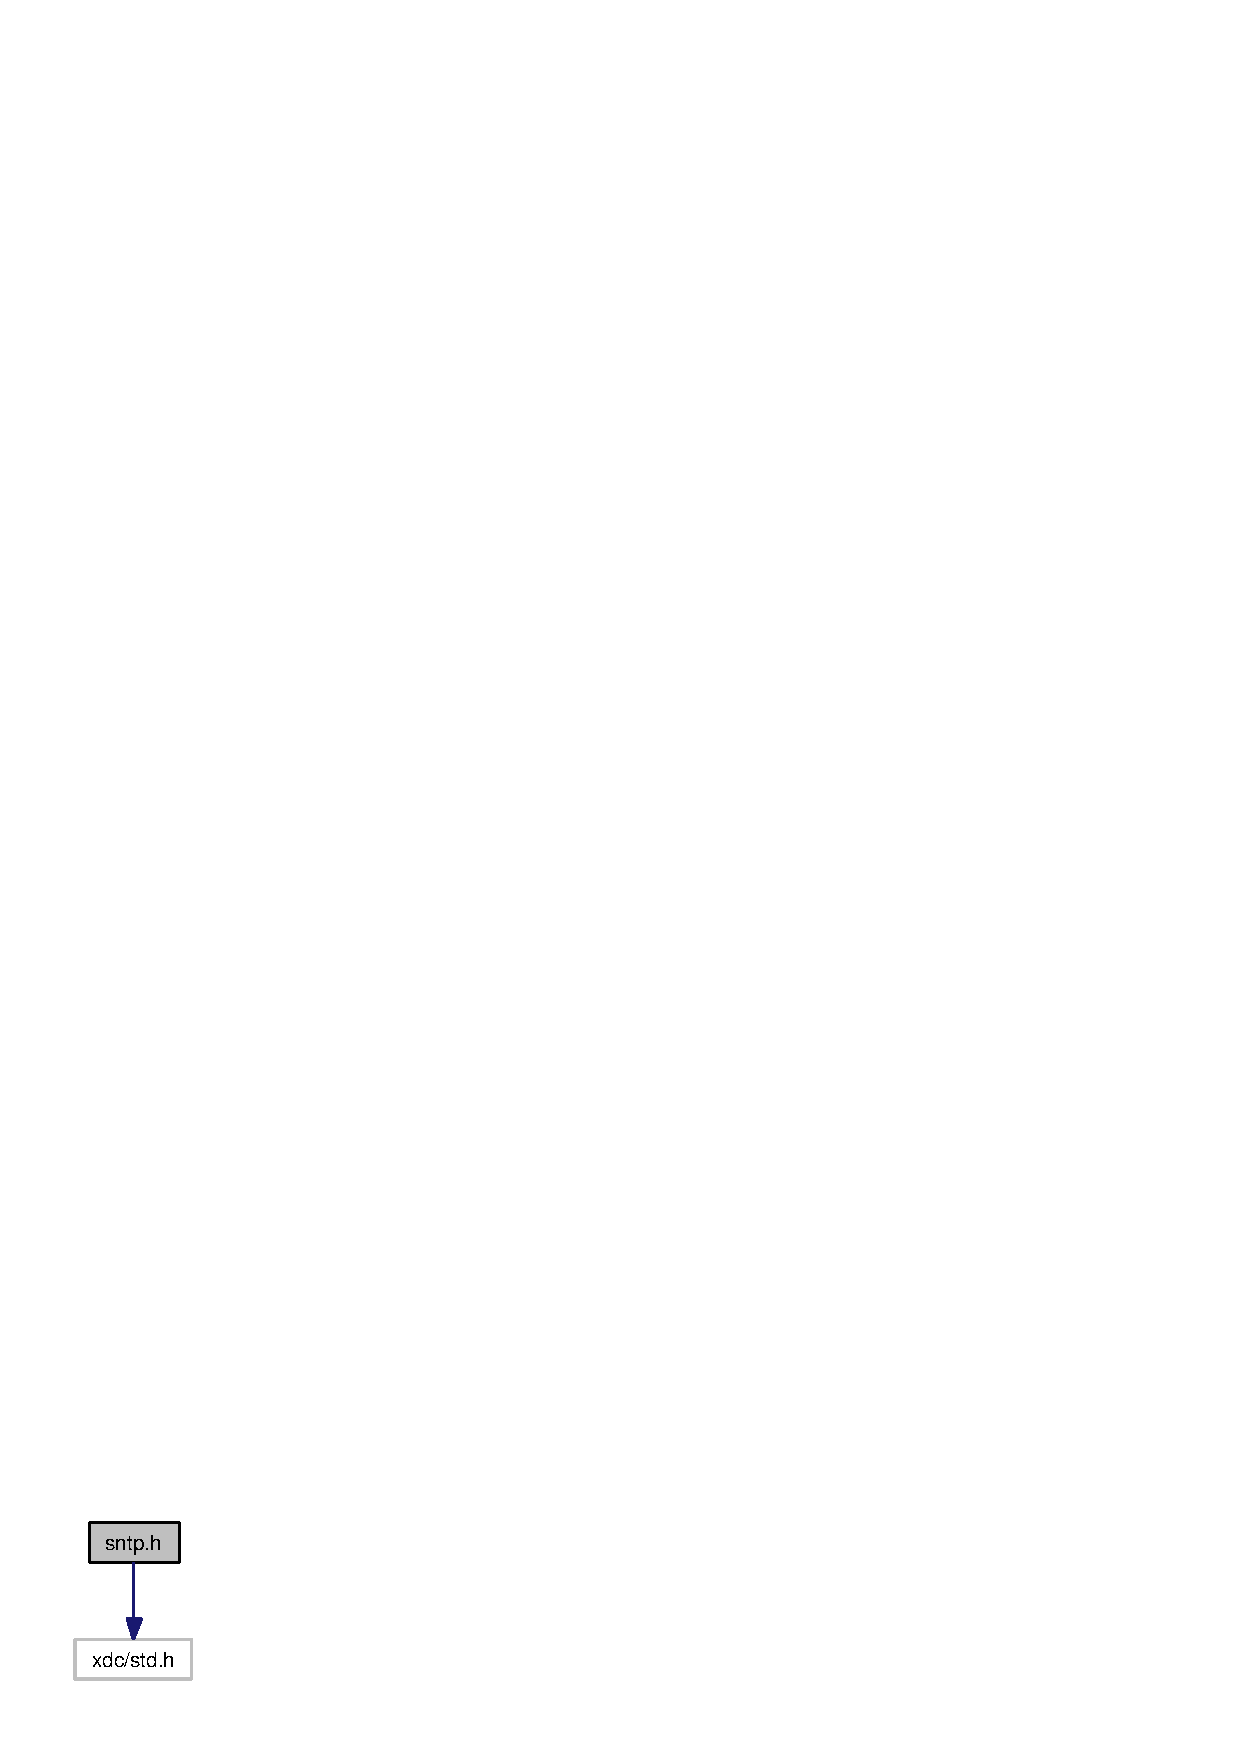
\includegraphics[width=93pt]{sntp_8h__incl}
\end{center}
\end{figure}
\subsubsection*{Functions}
\begin{DoxyCompactItemize}
\item 
int \hyperlink{sntp_8h_a0b8765ce6d90d7d171d740b2eedde328}{S\+N\+T\+P\+\_\+start} (uint32\+\_\+t($\ast$get)(void), void($\ast$set)(uint32\+\_\+t newtime), size\+\_\+t stacksize)
\begin{DoxyCompactList}\small\item\em Initialize and start the S\+N\+T\+P client Task. \end{DoxyCompactList}\item 
void \hyperlink{sntp_8h_aaab818e780a8ec9e87aa39a4d9a31f89}{S\+N\+T\+P\+\_\+stop} (void)
\begin{DoxyCompactList}\small\item\em Stops the S\+N\+T\+P client Task and frees resources used by the module. \end{DoxyCompactList}\item 
void \hyperlink{sntp_8h_a34409ecc254ee5abf525c69909d3df59}{S\+N\+T\+P\+\_\+setservers} (struct sockaddr $\ast$servers, unsigned int numservers)
\begin{DoxyCompactList}\small\item\em Initializes or updates the list of N\+T\+P servers to communicate with. \end{DoxyCompactList}\end{DoxyCompactItemize}


\subsubsection{Function Documentation}
\index{sntp.\+h@{sntp.\+h}!S\+N\+T\+P\+\_\+start@{S\+N\+T\+P\+\_\+start}}
\index{S\+N\+T\+P\+\_\+start@{S\+N\+T\+P\+\_\+start}!sntp.\+h@{sntp.\+h}}
\paragraph[{S\+N\+T\+P\+\_\+start}]{\setlength{\rightskip}{0pt plus 5cm}int S\+N\+T\+P\+\_\+start (
\begin{DoxyParamCaption}
\item[{uint32\+\_\+t($\ast$)(void)}]{get, }
\item[{void($\ast$)(uint32\+\_\+t newtime)}]{set, }
\item[{size\+\_\+t}]{stacksize}
\end{DoxyParamCaption}
)}\label{sntp_8h_a0b8765ce6d90d7d171d740b2eedde328}


Initialize and start the S\+N\+T\+P client Task. 

Called to create and start S\+N\+T\+P client Task and Semaphores. User must pass in pointers to functions for getting and setting the current time.

The S\+N\+T\+P client Task\textquotesingle{}s stacksize is configurable via the stacksize parameter.

Passing a value of 0 for the stack parameter causes the Task to be created with a default value. Passing a value $>$ 0 causes the Task to be created using that value for the stack size. When a value $>$ 0 is passed, it is the application developer\textquotesingle{}s responsiblity to choose an appropriate stack size. If this is not done, stack overflow or other undesirable behavior may occur.

The priority of S\+N\+T\+P\+\_\+synctime is set to 1 and is not configurable.


\begin{DoxyParams}{Parameters}
{\em get} & A pointer to a function that returns the number of seconds since January 1, 1970\\
\hline
{\em set} & A pointer to a function that sets the time to the supplied value\\
\hline
{\em stacksize} & Stack size to use for the S\+N\+T\+P client Task. Passing a value of 0 allows a default to be used.\\
\hline
\end{DoxyParams}
\begin{DoxyReturn}{Returns}
0 on failure and 1 on success 
\end{DoxyReturn}
\index{sntp.\+h@{sntp.\+h}!S\+N\+T\+P\+\_\+stop@{S\+N\+T\+P\+\_\+stop}}
\index{S\+N\+T\+P\+\_\+stop@{S\+N\+T\+P\+\_\+stop}!sntp.\+h@{sntp.\+h}}
\paragraph[{S\+N\+T\+P\+\_\+stop}]{\setlength{\rightskip}{0pt plus 5cm}void S\+N\+T\+P\+\_\+stop (
\begin{DoxyParamCaption}
\item[{void}]{}
\end{DoxyParamCaption}
)}\label{sntp_8h_aaab818e780a8ec9e87aa39a4d9a31f89}


Stops the S\+N\+T\+P client Task and frees resources used by the module. 

\index{sntp.\+h@{sntp.\+h}!S\+N\+T\+P\+\_\+setservers@{S\+N\+T\+P\+\_\+setservers}}
\index{S\+N\+T\+P\+\_\+setservers@{S\+N\+T\+P\+\_\+setservers}!sntp.\+h@{sntp.\+h}}
\paragraph[{S\+N\+T\+P\+\_\+setservers}]{\setlength{\rightskip}{0pt plus 5cm}void S\+N\+T\+P\+\_\+setservers (
\begin{DoxyParamCaption}
\item[{struct sockaddr $\ast$}]{servers, }
\item[{unsigned int}]{numservers}
\end{DoxyParamCaption}
)}\label{sntp_8h_a34409ecc254ee5abf525c69909d3df59}


Initializes or updates the list of N\+T\+P servers to communicate with. 

Must call \hyperlink{sntp_8h_a0b8765ce6d90d7d171d740b2eedde328}{S\+N\+T\+P\+\_\+start()} first. This function is used to set the list of N\+T\+P servers initially, or to update the list of servers at a later point in the application run.


\begin{DoxyParams}{Parameters}
{\em servers} & A pointer to a contiguous block of memory which contains a list of sockaddr\+\_\+in and/or sockaddr\+\_\+in6 structures\\
\hline
{\em numservers} & The number of servers (structs) contained in the server list \\
\hline
\end{DoxyParams}

%--- End generated contents ---

% Index
\backmatter
\newpage
\phantomsection
\clearemptydoublepage
\addcontentsline{toc}{section}{Index}
\printindex

\end{document}
